% >8-----------------------------------------------------------------------------------------------------------------8<

\chapter{Transformando uma EDO Genérica em um Sistema Matriz-vetor}
\section{Definição da Formulação Forte}

  Dada uma função $f : [0,1] \to \mathbb{R}$ e constantes $\alpha > 0$, $\beta \geq 0$ e $\gamma \geq 0$, queremos encontrar a função $u : [0,1] \to \mathbb{R}$ tal que:

  \begin{center}
    $(S) = \begin{cases}
      -\alpha u_{xx}(x) + \beta u(x) + \gamma u_{x}(x) = f(x) \\
      \\
      u(0) = u(1) = 0
    \end{cases}$
  \end{center}

  Sendo $(S)$ conhecido como a formulação forte do problema.

\section{Transição da Formulação Forte para a Formulação Fraca}

Nesse momento iremos realizar uma série de manipulações algébricas para deixá-la em um formato mais próximo de uma formulação fraca, que é mais adequada para análise teórica e para implementação numérica.

Visto que $-\alpha u_{xx}(x) + \beta u(x) + \gamma u_{x}(x) = f(x)$, podemos multiplicar ambos os lados por uma função $v(x)$ tal que $v(1) = v(0) = 0$ que nos ajude a eliminar a segunda derivada $u_{xx}$:

\begin{align*}
  -\alpha u_{xx}(x) + \beta u(x) + \gamma u_{x}(x) &= f(x)  \\
  \left[-\alpha u_{xx}(x) + \beta u(x) + \gamma u_{x}(x)\right]v(x) &= f(x)v(x) \\
  -\alpha u_{xx}(x)v(x) + \beta u(x)v(x) + \gamma u_{x}(x)v(x) &= f(x)v(x)\\
  \int^{1}_{0} \left[-\alpha u_{xx}(x)v(x) + \beta u(x)v(x) + \gamma u_{x}(x)v(x)\right] dx &= \int^{1}_{0} f(x)v(x) dx\\
  \int^{1}_{0} -\alpha u_{xx}(x)v(x) dx + \int^{1}_{0} \beta u(x)v(x) dx + \int^{1}_{0} \gamma u_{x}(x)v(x) dx &= \int^{1}_{0} f(x)v(x) dx
\end{align*}

Sabemos que dadas funções $f$ e $g$:

\begin{align*}
  \int f(x)g'(x)dx &= f(x)g(x) - \int f'(x)g(x)dx
\end{align*}

Logo, realizando a integração por partes no primeiro termo na equação:

\begin{align*}
-\alpha \left[u_{x}(x)v(x) \bigg|^{1}_{0} - \int^{1}_{0} u_{x}(x)v_{x}(x) dx\right] + \int^{1}_{0} \beta u(x)v(x) dx + \int^{1}_{0} \gamma u_{x}(x)v(x) dx &= \int^{1}_{0} f(x)v(x) dx\\
-\alpha \left[(u_{x}(1)v(1) - u_{x}(0)v(0)) - \int^{1}_{0} u_{x}(x)v_{x}(x) dx\right] + \int^{1}_{0} \beta u(x)v(x) dx + \int^{1}_{0} \gamma u_{x}(x)v(x) dx &= \int^{1}_{0} f(x)v(x) dx\\
-\alpha \left[\cancel{(u_{x}(1)v(1) - u_{x}(0)v(0))} - \int^{1}_{0} u_{x}(x)v_{x}(x) dx\right] + \int^{1}_{0} \beta u(x)v(x) dx + \int^{1}_{0} \gamma u_{x}(x)v(x) dx  &= \int^{1}_{0} f(x)v(x) dx\\
\alpha \int^{1}_{0} u_{x}(x)v_{x}(x) dx + \beta \int^{1}_{0} u(x)v(x) dx + \gamma \int^{1}_{0} u_{x}(x)v(x) dx &= \int^{1}_{0} f(x)v(x) dx\\
\end{align*}

\section{Definição da Formulação Fraca}

  \textbf{Definição}: Pelo restante do documento, considere que uma função $g$ é ``suficientemente suave'' se ela respeitar:

  \begin{itemize}
    \item $g$ é contínua em todo o domínio;
    \item $g$ possui derivadas contínuas até a ordem necessária;
  \end{itemize}

Seja $H$ um espaço de funções formado por funções $u$ suficientemente suaves que satisfazem $(W)$ e as condições de contorno $u(0) = u(1) = 0$. Seja $V$ um espaço das funções de teste, composto por funções $v$ suficientemente suaves e que satisfazem as condições de contorno $v(0) = v(1) = 0$.

Dados $\alpha > 0$, $\beta \geq 0$, $\gamma \geq 0$ e uma função $f : [0,1] \to \mathbb{R}$, precisamos determinar $u : [0,1] \to \mathbb{R}, u \in H$, tal que, $\forall v \in V$,

\[(W) = \begin{cases} \alpha \displaystyle\int^{1}_{0} u_{x}(x)v_{x}(x) dx + \beta \int^{1}_{0} u(x)v(x) dx + \gamma \int^{1}_{0} u_{x}(x)v(x) dx = \int^{1}_{0} f(x)v(x) dx.\\
  \\
  u(0) = u(1) = 0
\end{cases}\]


\section{Definição do Problema Aproximado pelo Método de Galerkin}

O método de Galerkin consiste em aproximar o espaço das soluções por um subespaço de dimensão finita para encontrarmos uma solução aproximada que satisfaça a formulação fraca do problema dentro de um subespaço apropriado, permitindo a construção de uma solução computacionalmente viável. Sendo assim:

Seja $H^h$ um espaço de funções finito-dimensional composto por funções $u^h$ suficientemente suaves que satisfazem $(W)$ e as condições de contorno $u^h(0) = u^h(1) = 0$. Analogamente, seja $V^h$ um espaço de funções finito-dimensional das funções de teste, formado por funções $v^h$ suficientemente suaves que também atendem às condições de contorno $v^h(0) = v^h(1) = 0$.

Precisamos determinar $u^h \in H^h$ tal que, $\forall v^h \in V^h$,

\[\begin{cases} \displaystyle\int^{1}_{0} f(x)v^{h}(x) dx = \alpha \int^{1}_{0} u^{h}_{x}(x)v^{h}_{x}(x) dx + \beta \int^{1}_{0} u^{h}(x)v^{h}(x) dx + \gamma \int^{1}_{0} u^{h}_{x}(x)v^{h}(x) dx. \\
  \\
  u(0) = u(1) = 0
\end{cases}\]

\section{Transição do Problema Aproximado para a Forma Matriz-vetor}

Visto que $u^h \in H^h$, podemos tomar $u^h$ como combinação linear das funções da base de $H^h$.

Seja \[u^h(x) = \sum_{j=1}^{m} \varphi_j(x) c_j.\]

Logo, temos que:

\[u_{x}^h(x) = \sum_{j=1}^{m} \varphi_{xj}(x)c_j\]

Substituindo ambos em nossa equação:

\begin{align*}
\alpha \int_{0}^{1} \sum_{j=1}^{m} \varphi_{xj}(x) c_j v^h_x(x)dx + \beta \int_{0}^{1} \sum_{j=1}^{m} \varphi_j(x)c_j v^h(x)dx + \gamma \int_{0}^{1} \sum_{j=1}^{m} \varphi_{xj}(x)c_j v^h(x)dx &= \int_{0}^{1} f(x) v^h(x)dx\\
\sum_{j=1}^{m} c_j \left[ \alpha \int_{0}^{1} \varphi_{xj}(x)  v^h_x(x)dx + \beta \int_{0}^{1} \varphi_j(x) v^h(x)dx + \gamma \int_{0}^{1} \varphi_{xj}(x) v^h(x)dx \right] &= \int_{0}^{1} f(x) v^h(x)dx
\end{align*}

  Veja que podemos tomar $v^h(x)$ como sendo qualquer função da base $V^h$.

  $v^h(x) = \varphi_i(x)$, $i \in \{1,\dots,m\}$, e $v^h_x(x) = \varphi_{xi}(x)$

\begin{align*}
  \sum_{j=1}^{m} c_j \left[ \alpha \int_{0}^{1} \varphi_{xj}(x) \varphi_{xi}(x) dx + \beta \int_{0}^{1} \varphi_j(x) \varphi_i(x)dx + \gamma \int_{0}^{1} \varphi_{xj}(x) \varphi_i(x)dx \right] &= \int_{0}^{1} f(x) \varphi_i(x)dx
\end{align*}

Veja que essa equação vale para $i \in \{1,\dots,m\}$. Dessa forma, podemos expressar nosso problema na forma matriz-vetor.

\section{Definição do Problema na Forma Matriz-Vetor}

Veja que podemos escrever a equação acima como um sistema de $m$ equações ao variarmos o valor de $i$:

\[\begin{cases}
  \displaystyle\sum_{j=1}^{m} c_j \left[ \alpha \int_{0}^{1} \varphi_{xj}(x) \varphi_{x1}(x) dx + \beta \int_{0}^{1} \varphi_j(x) \varphi_1(x)dx + \gamma \int_{0}^{1} \varphi_{xj}(x) \varphi_1(x)dx \right] = \int_{0}^{1} f(x) \varphi_1(x)dx \\
  \vdots\\
  \displaystyle\sum_{j=1}^{m} c_j \left[ \alpha \int_{0}^{1} \varphi_{xj}(x) \varphi_{xi}(x) dx + \beta \int_{0}^{1} \varphi_j(x) \varphi_i(x)dx + \gamma \int_{0}^{1} \varphi_{xj}(x) \varphi_i(x)dx \right] = \int_{0}^{1} f(x) \varphi_i(x)dx \\
  \vdots \\
  \displaystyle\sum_{j=1}^{m} c_j \left[ \alpha \int_{0}^{1} \varphi_{xj}(x) \varphi_{xm}(x) dx + \beta \int_{0}^{1} \varphi_j(x) \varphi_m(x)dx + \gamma \int_{0}^{1} \varphi_{xj}(x) \varphi_m(x)dx \right] = \int_{0}^{1} f(x) \varphi_m(x)dx
\end{cases}\]

E veja que podemos escrever esse sistema na forma matriz vetor:

\[\mathcal{K}\mathcal{C} = \mathcal{F}\]

\[
\begin{pmatrix}
  \mathcal{K}_{1,1} & ... & \mathcal{K}_{1,j} & ... & \mathcal{K}_{1,m} \\
  \vdots & \ddots & \vdots & \ddots & \vdots \\
  \mathcal{K}_{i,1} & ... & \mathcal{K}_{i,j} & ... & \mathcal{K}_{i,m} \\
  \vdots & \ddots & \vdots & \ddots & \vdots \\
  \mathcal{K}_{m,1} & ... & \mathcal{K}_{m,j} & ... & \mathcal{K}_{m,m}
\end{pmatrix}
\begin{pmatrix}
  \mathcal{C}_1 \\ \vdots \\ \mathcal{C}_i \\ \vdots \\ \mathcal{C}_m
\end{pmatrix}
=
\begin{pmatrix}
  \mathcal{F}_1 \\ \vdots \\ \mathcal{F}_i \\ \vdots \\ \mathcal{F}_m
\end{pmatrix}
\]

Tal que:

\begin{align*}
  \mathcal{K}_{i,j} &= \alpha \int_{0}^{1} \varphi_{xi}(x) \varphi_{xj}(x)dx + \beta \int_{0}^{1} \varphi_i(x) \varphi_j(x)dx + \gamma \int_{0}^{1} \varphi_i(x) \varphi_{xj}(x)dx \\
  \mathcal{F}_i &= \int_{0}^{1} f(x) \varphi_i(x) dx
\end{align*}

\section{Definindo uma Função Base}

Seja $x_1, \dots, x_m$ uma discretização do intervalo $[0, 1]$ tal que $\forall i \in \{1, \dots, m\}$, $x_{i+1} - x_{i} = h$. Além disso, considere $x_0 = 0$ e $x_{m+1} = 1$ como sendo os extremos do intervalo tal que $x_{m+1} - x_m = h$ e $x_1 - x_0 = h$.

Definiremos $\varphi_i(x)$ como:

\[\varphi_i(x) = \begin{cases}
  \dfrac{x - x_{i-1}}{h}, &\forall x \in [x_{i-1}, x_i] \\
  \dfrac{x_{i+1} - x}{h}, &\forall x \in [x_{i}, x_{i+1}] \\
  0 , &\forall x \notin [x_{i-1}, x_{i+1}]
\end{cases}\]

Observe que a função base $\varphi_i(x)$ é definida como uma função linear por partes intencionalmente de forma que a sua integração e derivação sejam simples. Além disso, $\varphi_i(x)$ é projetada para ser zero fora do intervalo $[x_{i-1},x_{i+1}]$, o que significa que cada função base afeta apenas dois ou três pontos consecutivos. Essa escolha reduz significativamente a complexidade do sistema linear, já que a matriz resultante terá muitas entradas nulas. Isso nos é benéfico pois então trabalharemos com matrizes esparsas, que são computacionalmente mais eficientes, tanto em termos de armazenamento quanto de tempo de processamento.

Perceba também que:

\[\varphi_i(x_i) = \dfrac{x_i - x_{i-1}}{h} = \dfrac{h}{h} = 1.\]

\begin{figure}[H]
  \centering
  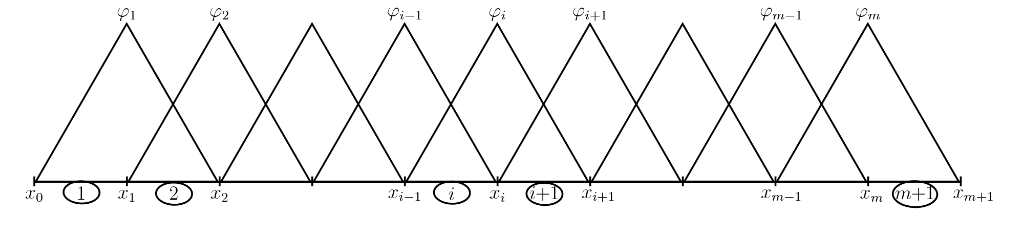
\includegraphics[width=0.9\linewidth]{phi-is.png}
  \caption{Definição das funções da base. Imagem de Bruno Alves do Carmo\cite{Bacarmo}.}
\end{figure}

% >8-----------------------------------------------------------------------------------------------------------------8<